\begin{frame}
  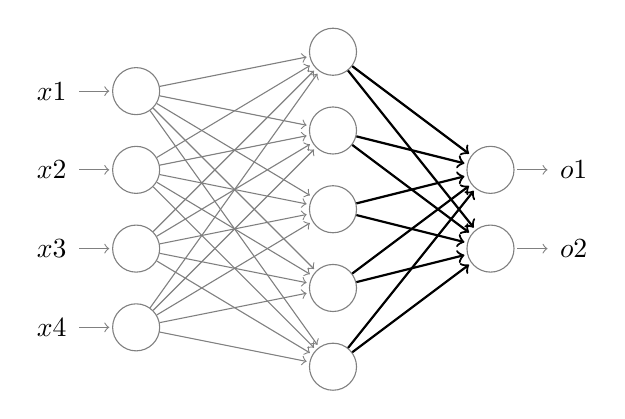
\begin{tikzpicture}[shorten >=1pt,->,draw=black!50, node distance=2.5cm]
    \tikzstyle{every pin edge}=[<-,shorten <=1pt]
    \tikzstyle{neuron}=[circle,draw,minimum size=17pt,inner sep=0pt]

    % input layer nodes
    \foreach \y in {1,...,4}
    \node[neuron, pin=left:$x\y$] (I-\y) at (0,-\y) {};

    % hidden layer nodes
    \foreach \y in {1,...,5}
    \path[yshift=0.5cm]
    node[neuron] (H-\y) at (2.5,-\y) {};

    % output layer node
    \foreach \y in {1,2}
    \path[yshift=-1cm]
    node[neuron,pin={[pin edge={->}]right:$o\y$}] (O-\y) at (4.5,-\y) {};

    % Connect every node in the input layer with every node in the
    % hidden layer.
    \foreach \src in {1,...,4}
    \foreach \dst in {1,...,5}
    \path (I-\src) edge (H-\dst);

    % Connect every node in the hidden layer with the output layer
    \foreach \src in {1,...,5}
    \foreach \dst in {1,2}
    \path[draw=black,thick] (H-\src) edge (O-\dst);
  \end{tikzpicture}
\end{frame}

\begin{frame}
  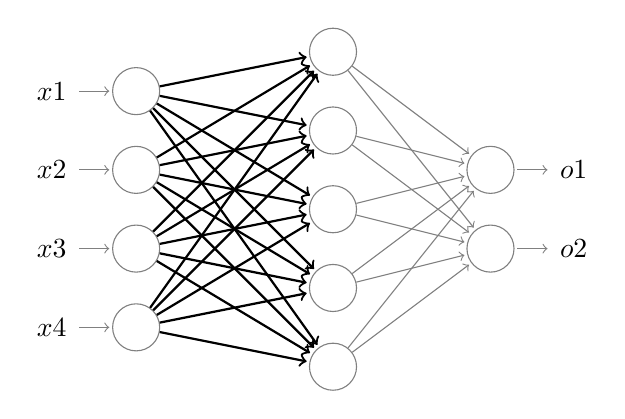
\begin{tikzpicture}[shorten >=1pt,->,draw=black!50, node distance=2.5cm]
    \tikzstyle{every pin edge}=[<-,shorten <=1pt]
    \tikzstyle{neuron}=[circle,draw,minimum size=17pt,inner sep=0pt]

    % input layer nodes
    \foreach \y in {1,...,4}
    \node[neuron, pin=left:$x\y$] (I-\y) at (0,-\y) {};

    % hidden layer nodes
    \foreach \y in {1,...,5}
    \path[yshift=0.5cm]
    node[neuron] (H-\y) at (2.5,-\y) {};

    % output layer node
    \foreach \y in {1,2}
    \path[yshift=-1cm]
    node[neuron,pin={[pin edge={->}]right:$o\y$}] (O-\y) at (4.5,-\y) {};

    % Connect every node in the input layer with every node in the
    % hidden layer.
    \foreach \src in {1,...,4}
    \foreach \dst in {1,...,5}
    \path[draw=black,thick] (I-\src) edge (H-\dst);

    % Connect every node in the hidden layer with the output layer
    \foreach \src in {1,...,5}
    \foreach \dst in {1,2}
    \path (H-\src) edge (O-\dst);
  \end{tikzpicture}
\end{frame}

\begin{frame}
  \begin{equation*}
    \begin{split}
      \frac{\partial E}{\partial w_{ij}} & = \frac{\partial E}{\partial o_j}
      \cdot \frac{\partial o_j}{\partial net_j} \cdot \frac{\partial
      net_j}{\partial w_{ij}}
    \end{split}
  \end{equation*}

  \begin{tikzpicture}[shorten >=1pt,->,draw=black!50, node distance=2.5cm]
    \tikzstyle{every pin edge}=[<-,shorten <=1pt]
    \tikzstyle{neuron}=[circle,draw,minimum size=17pt,inner sep=0pt]

    % input layer nodes
    \foreach \y in {1,...,4}
    \node[neuron, pin=left:$x\y$] (I-\y) at (0,-\y) {};

    % hidden layer nodes
    \foreach \y in {1,...,5}
    \path[yshift=0.5cm]
    node[neuron] (H-\y) at (2.5,-\y) {};

    % output layer node
    \path[yshift=-2cm]
    node[neuron,pin={[pin edge={->,draw=black,thick}]right:$o1$},
    draw=black,thick] (O-1) at (4.5,0) {$net_1$}
    node[neuron,pin={[pin edge={->}]right:$o2$}] (O-2) at (4.5,-1) {};

    % Connect every node in the input layer with every node in the
    % hidden layer.
    \foreach \src in {1,...,4}
    \foreach \dst in {1,...,5}
    \path (I-\src) edge (H-\dst);

    % Connect every node in the hidden layer with the output layer
    \foreach \src in {1,...,5}
    \foreach \dst in {1,2}
    \ifthenelse{\equal{\src}{4}\and\equal{\dst}{1}}
    {\path[draw=black,thick] (H-\src) edge node[below,right] {$w_{41}$} (O-\dst) {}}
    {\path (H-\src) edge (O-\dst)};
  \end{tikzpicture}
\end{frame}

\begin{frame}
  \begin{equation*}
    \begin{split}
      \frac{\partial net_j}{\partial w_{ij}} & = \frac{\partial}{\partial
    w_{ij}}(w_{0j} x_0 + \ldots + w_{ij} x_i + \ldots + w_{nj} x_n) \\
    & = x_i \\
    \frac{\partial o_j}{\partial net_j} & = \frac{\partial}{\partial
  w_{ij}}g(net_j) \\
  & = g(net_j) (1 - g(net_j)) \\
  & = oj(1 - oj) \\
      \frac{\partial E}{\partial o_j} & = \frac{\partial}{\partial o_j}(-y_j
      \log(o_j) - (1 - y_j) \log(1 - o_j))\\
      & = -y_j \frac{1}{o_j} - (1 - y_j) \frac{-1}{1 - o_j} \\
    \end{split}
  \end{equation*}
\end{frame}

\begin{frame}
  \begin{equation*}
    \begin{split}
      \frac{\partial E}{\partial w_{ij}} & = \frac{\partial E}{\partial o_j}
    \cdot \frac{\partial o_j}{\partial net_j} \cdot \frac{\partial
    net_j}{\partial w_{ij}} \\
    & = (-y_j \frac{1}{o_j} - (1 - y_j) \frac{-1}{1 - o_j}) oj(1 - o_j) x_i \\
    & = (-y_j \frac{1}{o_j} + \frac{1}{1 - o_j} - \frac{y_j}{1 - o_j}) o_j(1 - oj) x_i \\
    & = (-y_j \frac{1 - o_j}{o_j} + 1 - y_j) o_j x_i \\
    & = (-y_j (1 - o_j) + o_j - y_j o_j) x_i \\
    & = \underbrace{(o_j - y_j)}_{\delta_j} x_i \\
  \end{split}
\end{equation*}
\end{frame}

\begin{frame}[fragile]
  \begin{block}{Backpropagation}
    \begin{lstlisting}
def gradient(out, y, w):|\pause|
    L = len(out) - 1|\pause|
    x = add_bias(out[L - 1])|\pause|
    d = out[L] - y|\pause|
    grad = [x * transpose(d)]|\pause|
    ...
    \end{lstlisting}
  \end{block}
\end{frame}

\begin{frame}
  \begin{equation*}
    \begin{split}
      \frac{\partial E}{\partial w_{ij}} & = \frac{\partial E}{\partial o_j}
      \only<1>{\cdot \frac{\partial o_j}{\partial net_j} \cdot \frac{\partial
      net_j}{\partial w_{ij}}} \only<2>{o_j (1 - o_j) x_i}
    \end{split}
  \end{equation*}
  \begin{tikzpicture}[shorten >=1pt,->,draw=black!50, node distance=2.5cm]
    \tikzstyle{every pin edge}=[<-,shorten <=1pt]
    \tikzstyle{neuron}=[circle,draw,minimum size=17pt,inner sep=0pt]

    % input layer nodes
    \foreach \y in {1,...,4}
    \node[neuron, pin=left:$x\y$] (I-\y) at (0,-\y) {};

    % hidden layer nodes
    \path[yshift=0.5cm]
    node[neuron] (H-1) at (2.5,-1) {}
    node[neuron] (H-2) at (2.5,-2) {}
    node[neuron] (H-3) at (2.5,-3) {}
    node[neuron,draw=black,thick,label=right:{$o4$}] (H-4) at (2.5,-4) {$net_4$}
    node[neuron] (H-5) at (2.5,-5) {};

    % output layer node
    \path[yshift=-2cm]
    node[neuron,pin={[pin edge={->}]right:$o1$}] (O-1) at (4.5,0) {}
    node[neuron,pin={[pin edge={->}]right:$o2$}] (O-2) at (4.5,-1) {};

    % Connect every node in the input layer with every node in the
    % hidden layer.
    \foreach \src in {1,...,4}
    \foreach \dst in {1,...,5}
    \ifthenelse{\equal{\src}{2}\and\equal{\dst}{4}}
    {\path[draw=black,thick] (I-\src) edge node[above] {$w_{24}$} (H-\dst)}
    {\path (I-\src) edge (H-\dst)};

    % Connect every node in the hidden layer with the output layer
    \foreach \src in {1,...,5}
    \foreach \dst in {1,2}
    \path (H-\src) edge (O-\dst);
  \end{tikzpicture}
\end{frame}

\begin{frame}
  \begin{equation*}
    \frac{\partial E}{\partial out_{j}} = \displaystyle\sum_k{\left(
        \only<1,2>{\frac{\partial E}{\partial net_k}}
        \only<3,4>{\delta_k}
        \only<1>\cdot
        \only<1>{\frac{\partial net_k}{\partial out_j}}
    \only<2,3,4>{w_{jl}}\right)} \onslide<4>{= w_j \cdot \delta}
  \end{equation*}
  \begin{tikzpicture}[shorten >=1pt,->,draw=black!50, node distance=2.5cm]
    \tikzstyle{every pin edge}=[<-,shorten <=1pt]
    \tikzstyle{neuron}=[circle,draw,minimum size=17pt,inner sep=0pt]

    % input layer nodes
    \foreach \y in {1,...,4}
    \node[neuron, pin=left:$x\y$] (I-\y) at (0,-\y) {};

    % hidden layer nodes
    \path[yshift=0.5cm]
    node[neuron] (H-1) at (2.5,-1) {}
    node[neuron] (H-2) at (2.5,-2) {}
    node[neuron] (H-3) at (2.5,-3) {}
    node[neuron,draw=black,thick,label=right:{$o4$}] (H-4) at (2.5,-4) {}
    node[neuron] (H-5) at (2.5,-5) {};

    % output layer node
    \foreach \y in {1,2}
    \path[yshift=-1cm]
    node[neuron,draw=black,thick,pin={[pin edge={->,draw=black,thick}]right:$o\y$}] (O-\y) at
    (4.5,-\y) {$net_\y$};

    % Connect every node in the input layer with every node in the
    % hidden layer.
    \foreach \src in {1,...,4}
    \foreach \dst in {1,...,5}
    \path (I-\src) edge (H-\dst);

    % Connect every node in the hidden layer with the output layer
    \foreach \src in {1,...,5}
    \foreach \dst in {1,2}
    \ifthenelse{\equal{\src}{4}}
    {\path[draw=black,thick] (H-\src) edge (O-\dst)}
    {\path (H-\src) edge (O-\dst)};
  \end{tikzpicture}
\end{frame}

\begin{frame}
  \begin{equation*}
    \begin{split}
      \frac{\partial E}{\partial w_{ij}} & = \frac{\partial E}{\partial o_j}
      \cdot \frac{\partial o_j}{\partial net_j} \cdot \frac{\partial
      net_j}{\partial w_{ij}} \\
      & = \frac{\partial E}{\partial o_j} o_j (1 - o_j) x_i \\
      & = \underbrace{(\delta \cdot w_j) o_j (1 - o_j)}_{\delta} x_i \\
    \end{split}
  \end{equation*}
\end{frame}

\begin{frame}[fragile]
  \begin{block}{Backpropagation}
    \begin{lstlisting}
def gradient(out, y, w):
    L = len(out) - 1
    x = insert(out[L - 1], 0, 1, axis=0)
    d = out[L] - y
    grad = [x * transpose(d)]
|\pause|
    for l in range(len(out))[1:-1][::-1]:|\pause|
        d_out = w[l][1:] * d|\pause|
        d = multiply(d_out, multiply(out[l], 1 - out[l]))|\pause|
        x = add_bias(out[l - 1])|\pause|
        grad = [x * transpose(d)] + grad|\pause|
    return grad
    \end{lstlisting}
  \end{block}
\end{frame}
